\section{Complex pipelining}

Achieving high performance in pipelining introduces significant complexity, particularly when dealing with long latency or partially pipelined Floating Point Units (FPUs), multiple function and Memory Units (MUs), memory systems with variable access times, and precise exception handling.

A potential solution to these challenges is the complex in-order pipeline. This pipeline introduces a delay in the WB stage to ensure that all operations have the same latency to the WB stage. It avoids over-subscription of write ports, allowing one instruction to enter and exit each cycle. 
Furthermore, it enforces in-order instruction commitment, simplifying the implementation of precise exception handling.
\begin{figure}[H]
    \centering
    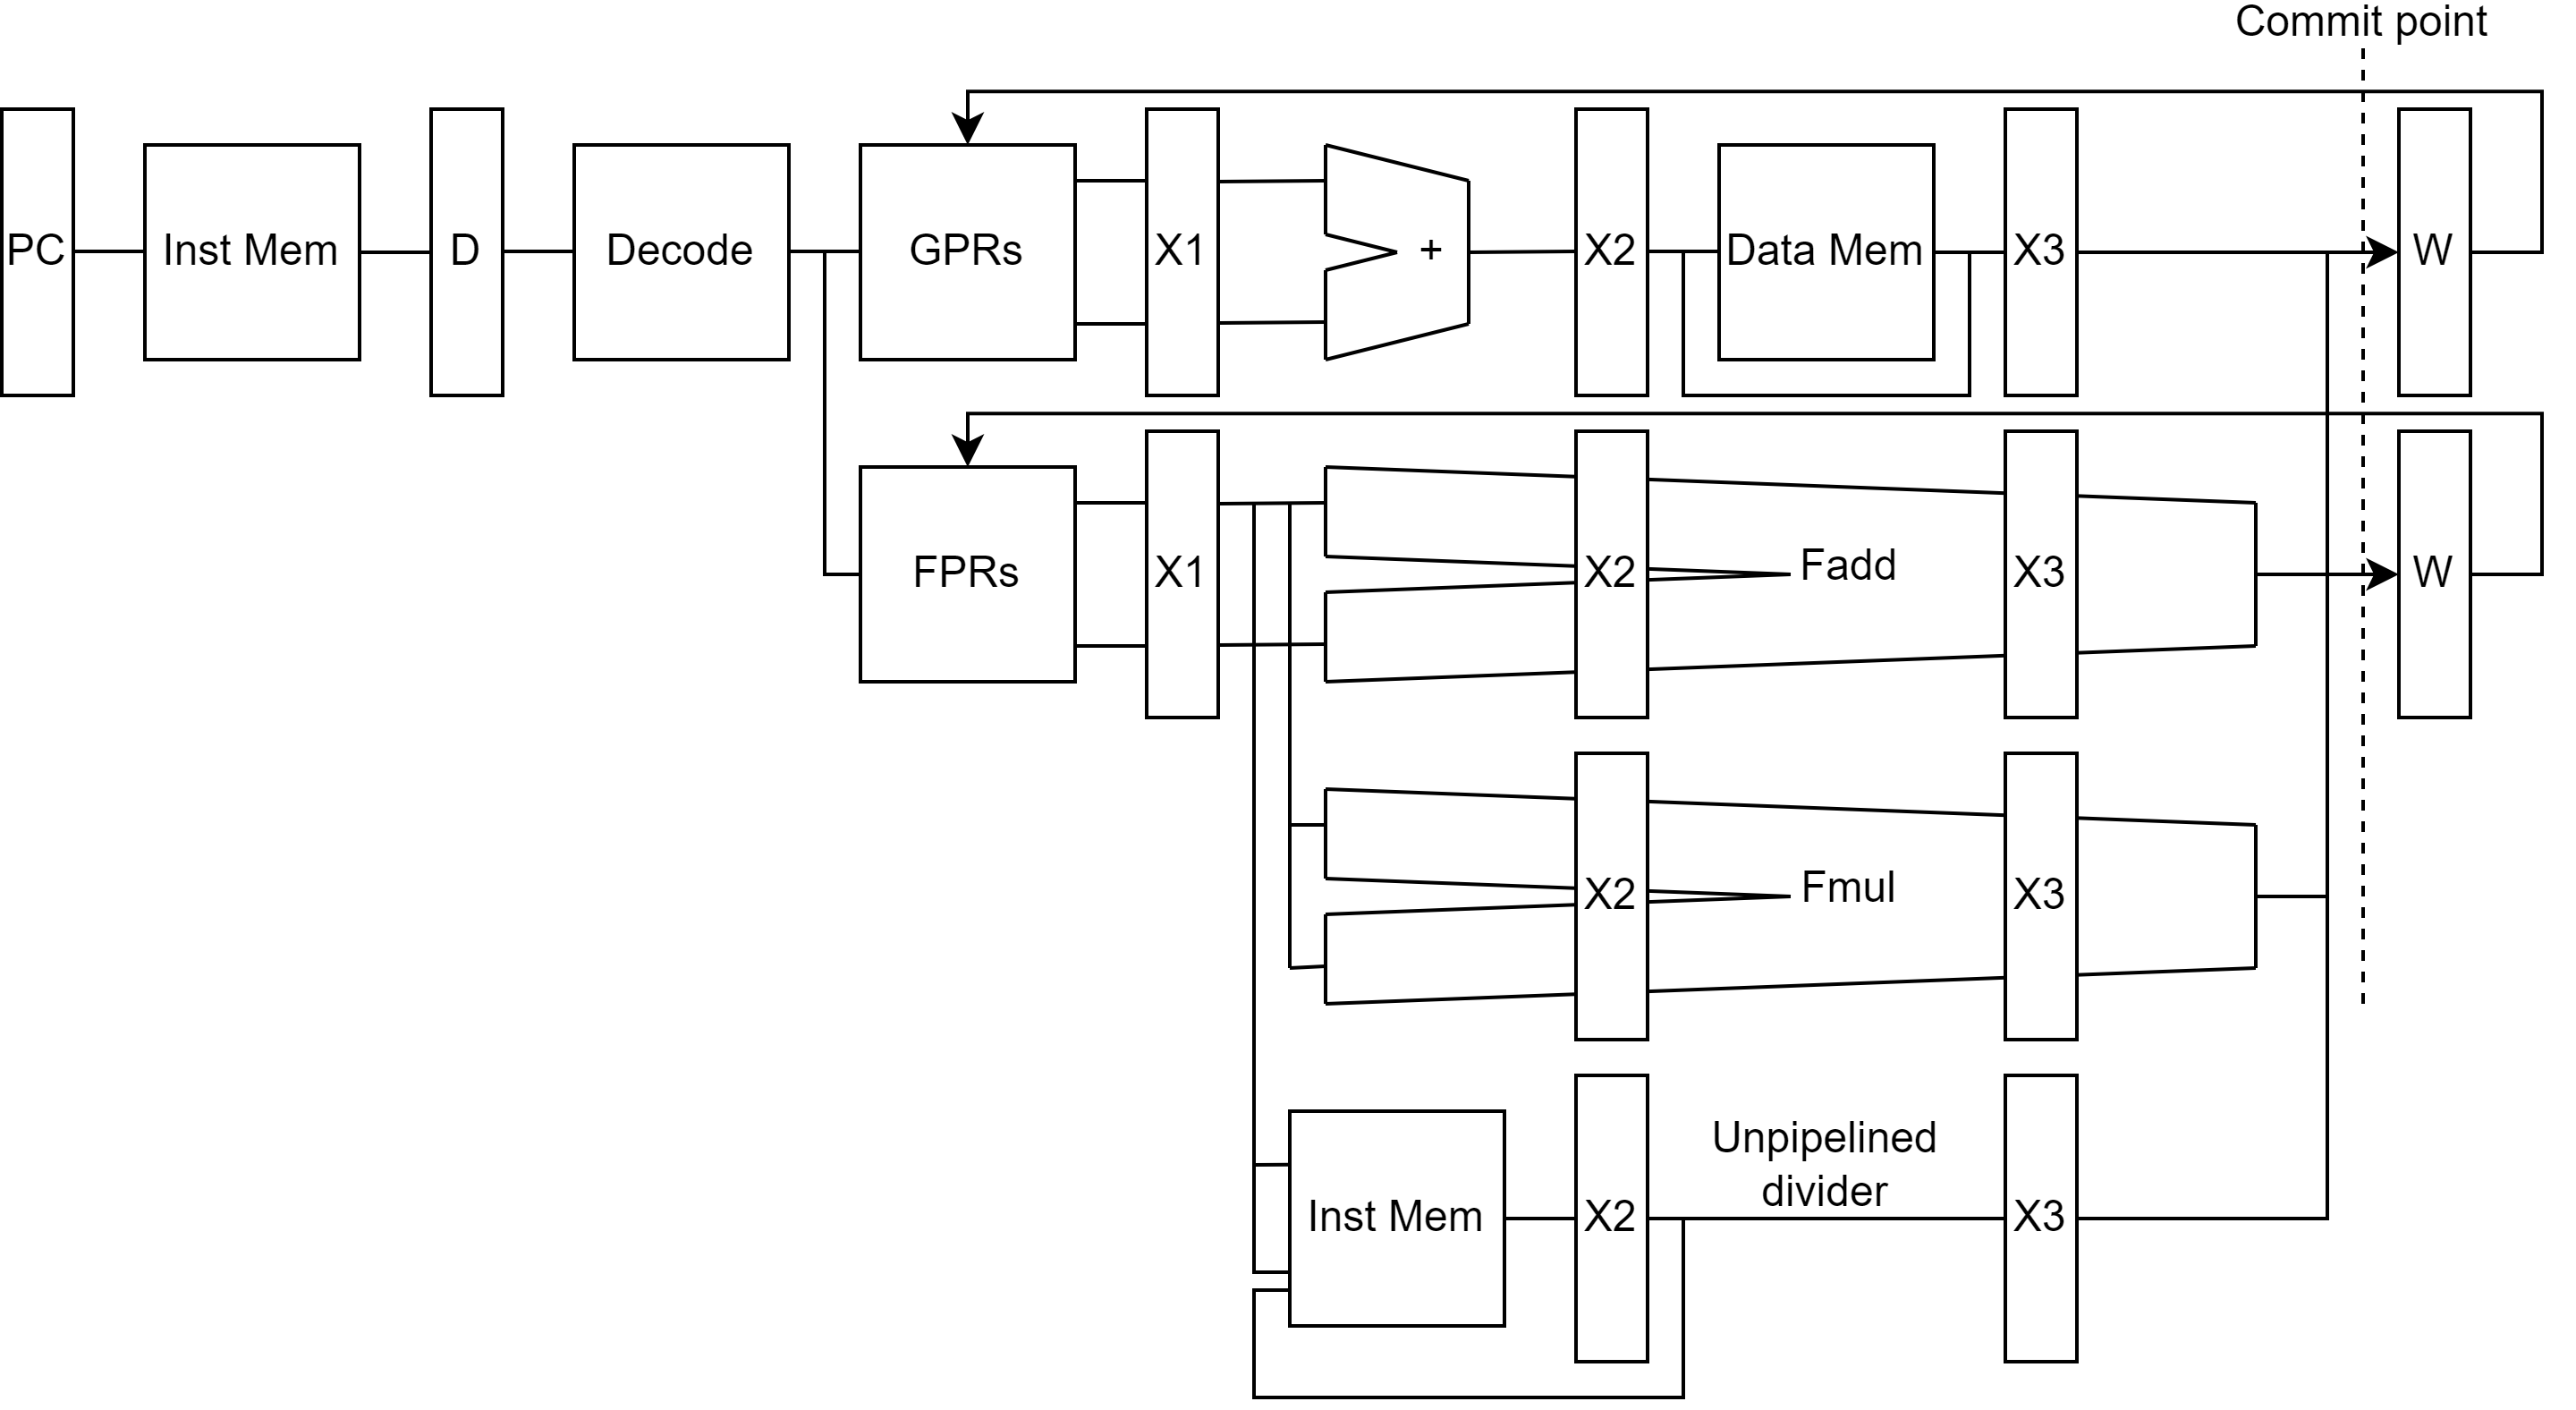
\includegraphics[width=0.5\linewidth]{images/ciop.png}
    \caption{Complex in order pipeline}
\end{figure}
However, several issues arise with this approach. 
Structural conflicts can occur during the execution stage if certain FPUs or MUs are not pipelined and take longer than one cycle. 
Structural conflicts also emerge at the WB stage because different functional units may have variable latencies. 
Additionally, out-of-order write hazards can occur due to these varying latencies.